\documentclass[UTF8]{ctexart}


\usepackage{tikz,mathpazo}
\usetikzlibrary{shapes.geometric, arrows}
\usetikzlibrary{calc}


\usepackage{listings}
%插入代码的配置
\definecolor{mygreen}{rgb}{0,0.6,0}
\definecolor{mygray}{rgb}{0.5,0.5,0.5}
\definecolor{mymauve}{rgb}{0.58,0,0.82}
\lstset{
 backgroundcolor=\color{lightgray},
 basicstyle = \footnotesize,
 breakatwhitespace = false,
 breaklines = true,
 captionpos = b,
 commentstyle = \color{mygreen}\bfseries,
 extendedchars = false,
 frame =shadowbox,
 framerule=0.5pt,
 keepspaces=true,
 keywordstyle=\color{blue}\bfseries, % keyword style
 language = C++,                     % the language of code
 otherkeywords={string},
 numbers=left,
 numbersep=5pt,
 numberstyle=\tiny\color{mygray},
 rulecolor=\color{black},
 showspaces=false,
 showstringspaces=false,
 showtabs=false,
 stepnumber=1,
 stringstyle=\color{mymauve},        % string literal style
 tabsize=2,
 title=\lstname
}



\usepackage{geometry}
\geometry{left=2cm, right=2cm, top=2cm, bottom=2cm}

%得到引用的标题内容
\usepackage{nameref}

%添加首行缩进,两个字符
\usepackage{indentfirst}
\setlength{\parindent}{2em}

%多行公式一个编号
\usepackage{amsmath}

%文献引用,标准类型为plain
%\usepackage[hyperref=true,backend=biber,sorting=none,backref=true]{biblatex}
%\addbibresource{ref.bib}
\bibliographystyle{plain}
\usepackage{cite}

\pagestyle{plain}


\usepackage{graphicx}

%超链接
\usepackage[linkcolor=yellow,citecolor=red,backref=page]{hyperref}
\hypersetup{
bookmarks=true,
colorlinks=true,
linkcolor=black
}

%引入了一些改进的数学环境,如align
\usepackage{amsmath}

\title{线性表编程作业}
%\author{姓名:鲁国锐 \protect\newline
%\and 学号:17020021031 \\
%\and 专业:电子信息科学与技术}
\author{姓名:寇一笑 \\
\and 学号:18020024016\\
\and 姓名:安皓源 \\
\and 学号:18020022001\\
}

\begin{document}
	\maketitle
	\renewcommand{\contentsname}{Contents}
	\tableofcontents
	\newpage
	
	\hypersetup{
	bookmarks=true,
	colorlinks=true,
	linkcolor=red,
	urlcolor=blue
	}
\section{第一题}
	\subsection{实验目的和内容}
	\subsubsection{题目描述}
    已知两个非降序的双向链表序列M1和M2\footnote{我们定义双向链表输入结尾是-1,这在题目中没有定义}, 请构造出它们合并后的非降序双向链表 ,并分析算法的时间复杂度。
%	\indent 祖玛是一款曾经风靡全球的游戏,其玩法是:在一条轨道上初始排列着若干个彩色珠子,其中任意三个相邻的珠子不会完全同色。此后,你可以发射珠子到轨道上并加入原有序列中。一旦有三个或更多同色的珠子变成相邻,它们就会立即消失。这类消除现象可能会连锁式发生,其间你将暂时不能发射珠子。

%\indent 开发商最近准备为玩家写一个游戏过程的回放工具。他们已经在游戏内完成了过程记录的功能,而回放功能的实现则委托你来完成。

%\indent 游戏过程的记录中,首先是轨道上初始的珠子序列,然后是玩家接下来所做的一系列操作。你的任务是,在各次操作之后及时计算出新的珠子序列。
\subsection{输入和输出说明}
	\subsubsection{输入}
    \indent 第一行是以空格为分隔的非降序数字序列,结尾是-1表示结束
    \indent 第二行是以空格为分隔的非降序数字序列,结尾是-1表示结束
%	\indent 第一行是一个由大写字母$’A’~’Z’$组成的字符串,表示轨道上初始的珠子序列,不同的字母表示不同的颜色。

%\indent 第二行是一个数字$n$,表示整个回放过程共有$n$次操作。

%\indent 接下来的$n$行依次对应于各次操作。每次操作由一个数字$k$和一个大写字母$\sum$描述,以空格分隔。其中,$\sum$为新珠子的颜色。若插入前共有$m$颗珠子,则$k\in[0, m]$表示新珠子嵌入之后(尚未发生消除之前)在轨道上的位序。
	\subsubsection{输出}
    输出一行以空格为分隔的非降序数字序列
%	\indent 输出共$n$行,依次给出各次操作(及可能随即发生的消除现象)之后轨道上的珠子序列。

%\indent 如果轨道上已没有珠子,则以“$-$”表示。
	\subsubsection{样例}
%	\begin{itemize}
%	\item 输入
%		\begin{itemize}
%			\item[ ]ACCBA
%			\item[ ]5
%			\item[ ]1 B
%			\item[ ]0 A
%			\item[ ]2 B
%			\item[ ]4 C
%			\item[ ]0 A
%		\end{itemize}
%	\item 输出
%		\begin{itemize}
%			\item[ ]ABCCBA
%			\item[ ]AABCCBA
%			\item[ ]AABBCCBA
%			\item[ ]-
%			\item[ ]A	
%		\end{itemize}
%	\end{itemize}
\begin{itemize}
    \item 输入
        \begin{itemize}
            \item[ ]2 3 4 -1
            \item[ ]2 3 4 5 -1
        \end{itemize}
    \item 输出
    \begin{itemize}
        \item[ ] 2 2 3 3 4 4 5
    \end{itemize}

        \item 输入
        \begin{itemize}
            \item[ ]2 3 3 -1
            \item[ ]2 2 2 -1
        \end{itemize}
    \item 输出
    \begin{itemize}
        \item[ ] 2 2 2 2 3 3
    \end{itemize}

    \item 输入
    \begin{itemize}
        \item[ ]-1
        \item[ ]-1
    \end{itemize}
    \item 输出
    \begin{itemize}
        \item[ ] exit(1)
    \end{itemize}
\end{itemize}
	
	\subsubsection{问题分析}
	\indent 根据题目,我们需要解决的问题有:
	\begin{itemize}
	\item[ ]
	\begin{enumerate}
%	\item 如何在插入后找出字符串中三个以上连续字符的位置;
%	\item 如何在进行消除后找出字符串中三个以上连续字符的位置;
    \item 如何建立双向链表
    \item 如何输出双向链表
    \item 如何将他们整合
	\end{enumerate}
	\end{itemize}	
	
%	\indent 至于消除的问题可以直接用模板库的函数来解决,所以不在我们要考虑的范围之内。	
	
	
	\subsection{解题思路}
\indent 本道题主程序非常简单,主要是需要实现三个函数的功能。首先是创建一个双链表,这可以通过单链表加上一个prior指针来实现。首先建立一个头结点,判断输入的第一个输入是否为-1,如果是则返回exit(1)。然后每次输入一个数字判断是否为-1,如果不是则新建一个结点并给它赋值并且加上双向的链子。\\
\indent 这里最重要的函数是merge函数,为了节省空间,我们在其中一个链表La进行原地操作。先设置第三个链表Lc的头结点为La的,然后判断la和lb的大小,将小的插入到双向链表Lc中,如果相等,则先插入La的,再插入Lb的,实现非降序排列。\\
\indent 最后是输出函数,我们对加上了对于空链表输出NULL,当指针遍历不为$NULL$时,依次输出数据域的值。
%	\indent 首先这道题需要注意的一点是,\textbf{给定的输入中可能有三个以上连续重复的字符},但根据以往玩游戏的经验,它并不会自动消除,而是需要人为地往里面再添加一个相同字符。所以我们不能每次都对整个字符串进行遍历。事实上,我们也不需要对整个字符串遍历,因为每次可能会出现消除的地方只会是插入后的位置以及消除后的“接口”位置。再进一步考虑,由于消除后后面的元素会向前填补,所以插入位置和消除后的“接口”处可以用同一个下标来表示。所以我们只用反复地考查插入位置附近是否有三个及以上连续相同字符并在符合条件的情况下进行消除。
%	
%	\indent 由此我们引出了解决本题时需要实现的两个函数:一个是$find$函数,用于考察插入位置附近是否有连续相同字符,返回该字符串的终止位置;一个是$ablat$,用于在符合条件时对find函数找出的字符串进行消除,并返回找出的字符串是否符合条件以确定是否需要再次调用$find$函数进行考察。
%	
%	\indent 首先我们来看一看$find$函数。为了实现其功能,我们需要对其传入参数插入位置的下标$start$以及目标字符串$balls$。我们再定义两个变量$left$和$right$,分别用来表示连续相同字符序列的起始下标和\textbf{终止下标的下一位}。我们先从$start$开始向左遍历,如果前一个元素等于当前元素,则令$left$减一;再从$start$开始向右遍历,如果下一个元素等于当前元素,则令$right$加一。注意不论是向左还是向右遍历,都不能超出字符串边界。另外还有一个小问题,我们调用$find$函数是为了找出满足条件的子序列的两头,我们可以直接返回$right$来输出末尾的下标,但起始的怎么办?如果是用一个数组来存放两个下标未免太不划算,所以这里我们在传参时直接传入$start$的引用,并在函数结束前把$left$的值赋给$start$即可。
%	
%	\indent 接下来我们再来看看$ablat$函数。为了实现其功能,我们需要传入起始下标$start$、终止下标$end$以及目标字符串$balls$。我们在定义一个变量$flag$,并令:
%	\begin{align}
%	flag = ((end - start) \geq 3) \label{flag}
%	\end{align}
%	
%	\indent 公式\ref{flag}的目的是用来判断$find$函数找出的字符串是否满足条件。如果是,则进行消除。最后再返回$flag$给主函数判断此次调用是否进行了消除操作,如果是,则还需调用$find$函数再次对$start$附近进行考查;反之则进入到下一次的插入操作当中去。
%	
%	\indent 到此算法的主要部分就分析完毕了,其余内容相对简单,在此不加赘述。
%	
%	\indent 另外在具体的实现上,我用了$vector$和$list$两种模板库进行实现(分别见list\ref{vec_code}和list\ref{list_code})。其中$vector$版我参照课本\cite{data_structure}实现了它的部分函数,并在清华大学的$Open\ Judge$上提交通过。而$list$版还未实现,所以还未经$Open\ Judge$的检验,在此只给出它的代码。
%	\section{算法设计}
%	见下页图\ref{vec_flowchart}。




%\begin{figure}[!htbp]
%	\centering
%	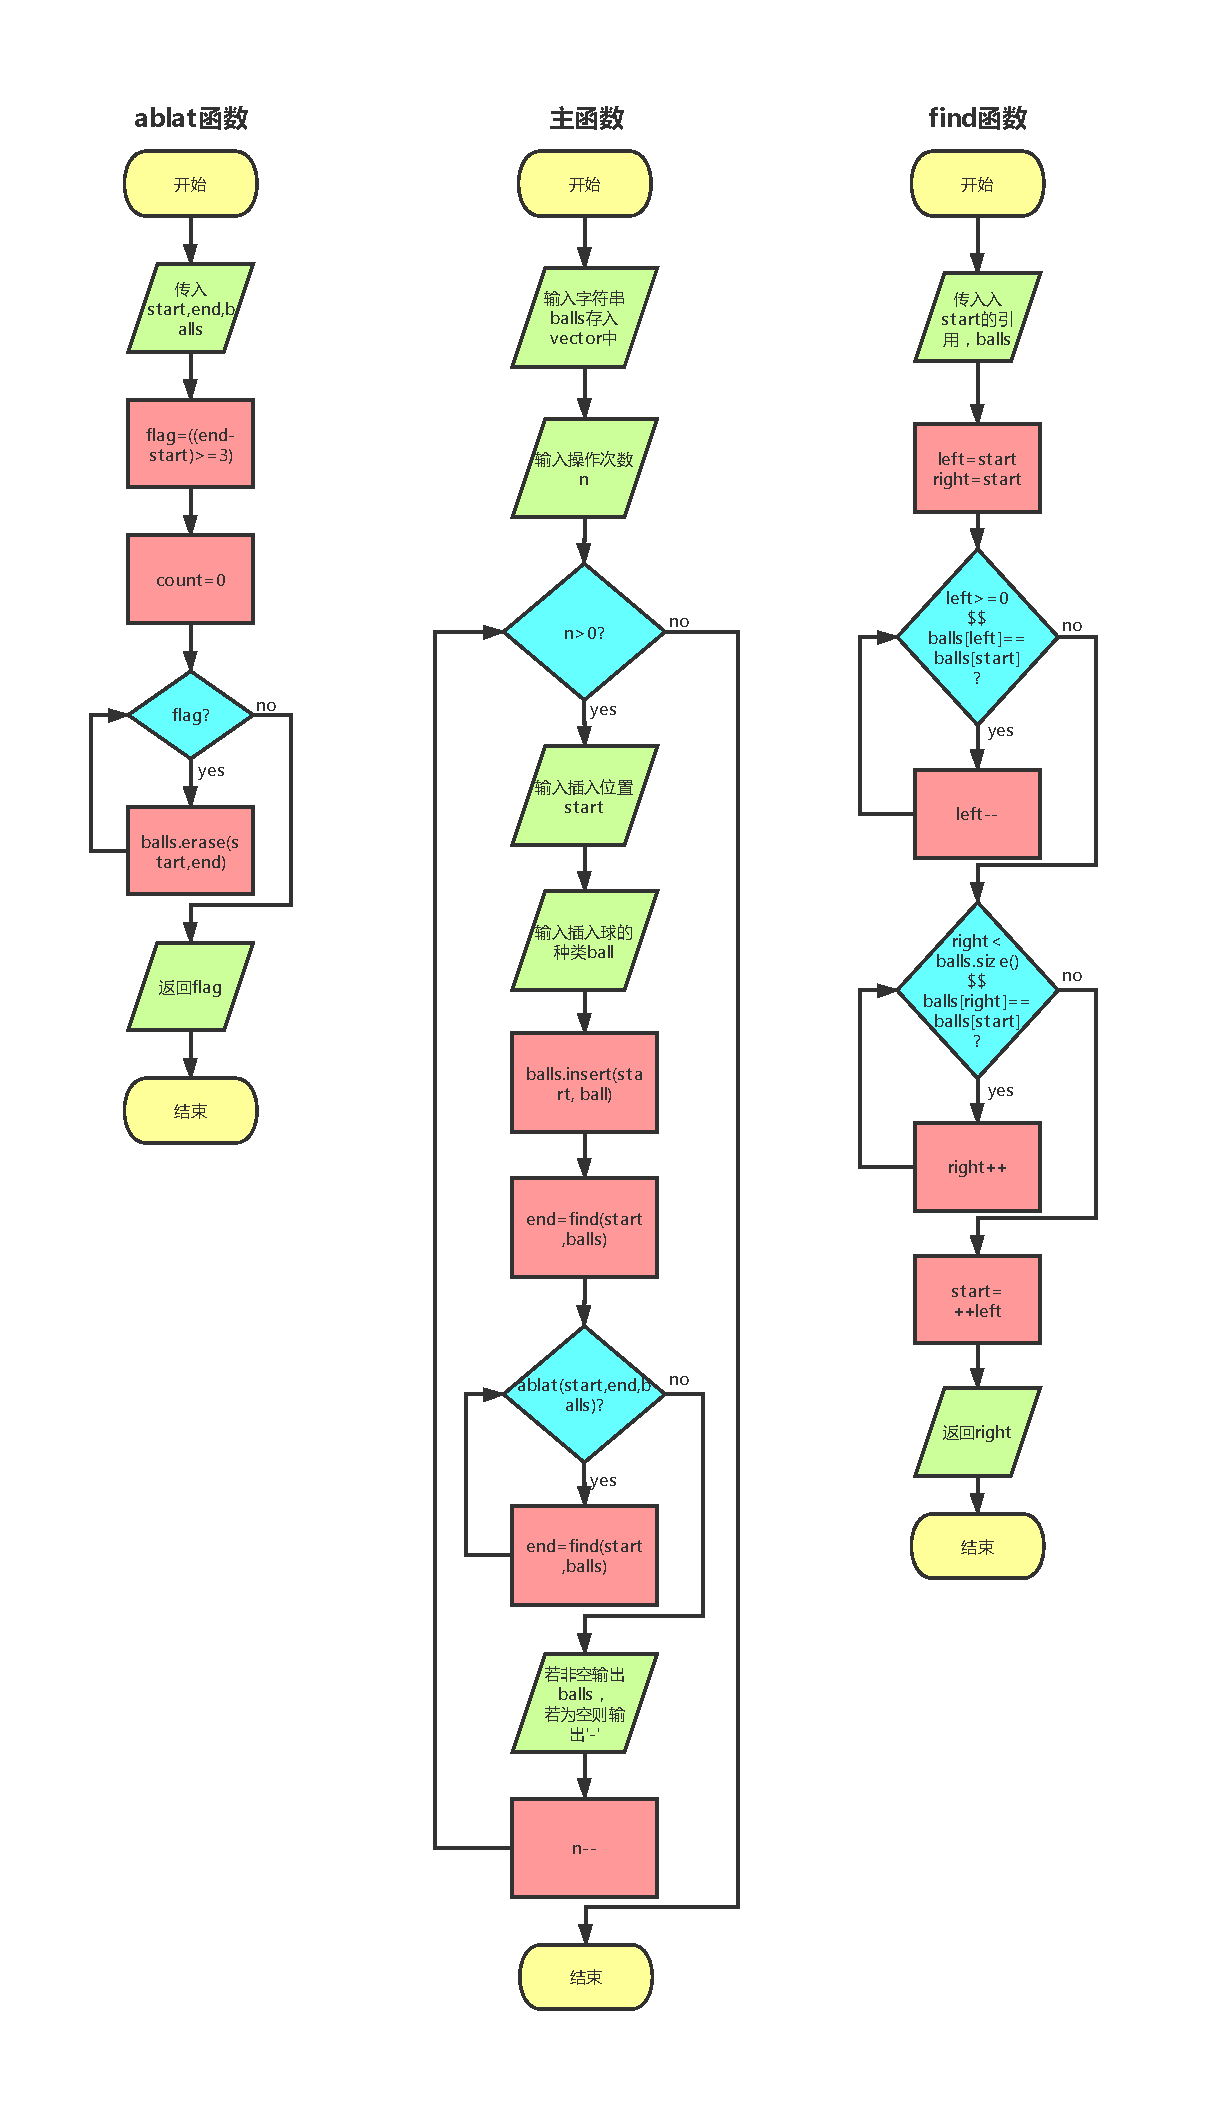
\includegraphics[scale=0.65]{zuma_flowchart.pdf}
%	\caption{vector版流程图}
%	\label{vec_flowchart}
%\end{figure}
%
%\newpage

	\subsection{实验代码及注释}
	\subsubsection{双向链表版}
	\begin{lstlisting}[language=C,caption={双向链表版本},label={dbl_code}]
#include <stdio.h>
#include <stdlib.h>
#include <malloc.h>

typedef int ElemType;
typedef struct node
{                      //链表结点
    ElemType data;     //结点数据域
    struct node *next, *prior; //结点指针域
} Listnode, *Linklist; //节点类型,节点指针

Linklist create_list(); //此处用了双向链表
Linklist merge_list(Linklist, Linklist); //声明合并的函数
void output_list(Linklist); //空链表将输出NULL

void main()
{
    Linklist L1, L2, L;
    printf("please input sequence1, end with -1:\t"); //本来想换行结尾,但是这样输入就是char了
    L1 = create_list();
    printf("please input sequence2, end with -1:\t");
    L2 = create_list();
    L = merge_list(L1, L2);
    printf("the result is:");
    output_list(L);
}

Linklist create_list() //创建链表并赋值
{
    int x;
    Linklist head, pa, pb; //头结点和两个指针,pb用来开辟空间,pa用来连接pb
    scanf("%d", &x);
    if(x==1) exit(1); //如果第一个输入为-1,异常退出
    head = (Linklist)malloc(sizeof(Listnode)); //定义头结点
    pa = head;
    while (x != -1)
    {
        pb = (Linklist)malloc(sizeof(Listnode));
        pb->data = x;
        pa->next = pb;
        pb->prior = pa;
        pa = pb;
        scanf("%d", &x);
    }
    pb->next = NULL; //指定最后一个为空,作为结束判断标志
    //创建双向链表
    return head; //返回头结点
}

Linklist merge_list(Linklist La, Linklist Lb)
{
    Linklist Lc, pa, pb, pc;
    Lc = La; //c链表的头结点,直接在a链表就地操作,降低空间复杂度
    pc = La;
    pa = La->next;
    pb = Lb->next;   //pa,pb是待插入结点的指针,pc是c链表待插入结点的前一个指针
    while (pa && pb) //while (pa!=NULL && pb!=NULL) La,Lb 链表不为空
    {
        if (pa->data < pb->data) //为了实现非降序排列需要进行分类讨论
        {
            pc->next = pa;
            pa->prior = pc;
            pc = pa;
            pa = pa->next;
        }
        if (pa->data > pb->data)
        {
            pc->next = pb;
            pb->prior = pc;
            pc = pb;
            pb = pb->next;
        }
        else //相等的话,就重复上述两个操作
        {
            pc->next = pa;
            pa->prior = pc;
            pc = pa;
            pa = pa->next;

            pc->next = pb;
            pb->prior = pc;
            pc = pb;
            pb = pb->next;
        }
    }
    if (pa != NULL)
    {
        pc->next = pa;
    }
    if (pb != NULL)
    {
        pc->next = pb;
    }
    // pa或者pb为空的话,直接将后续的链表加上去
    return Lc; //返回头结点
}

void output_list(Linklist s)
{
    s = s->next;
    if (s == NULL)
    {
        printf("NULL"); //空链表输出NULL
        return;         //直接结束,不执行下面代码
    }
    while (s != NULL)
    {
        printf("%d ", s->data);
        s = s->next;
    }
    printf("\n");
    return;
}
	\end{lstlisting}
	\subsubsection{双向循环链表版(未通过测试)}
	\begin{lstlisting}[language=C++,caption={双向循环链表版},label={dbl_circular_code}]
#include <stdio.h>
#include <stdlib.h>
#include <malloc.h>

typedef int Elemtype;
typedef struct node
{                      //链表结点
    Elemtype data;     //结点数据域
    struct node *next; //结点指针域
} Listnode, *Linklist; //节点类型,节点指针

typedef struct dnode
{
    Elemtype data;              //结点数据域
    struct dnode *prior, *next; //结点指针域
} DblNode, *DblList;            //节点类型,节点指针

DblList createDblList(); //此处用了双向循环链表
DblList mergeDblList(DblList, DblList);
void outputDblList(DblList); //空链表将输出NULL

void main()
{
    DblList L1, L2, L;
    printf("please input sequence1, end with -1:\t"); //本来想换行结尾,但是这样输入就是char了
    L1 = createDblList();
    printf("please input sequence2, end with -1:\t");
    L2 = createDblList();
    L = mergeDblList(L1, L2);
    printf("the result is:");
    outputDblList(L);
}

DblList createDblList() //建立双向循环链表
{
    DblList head, pa, pb;
    int x = 0;
    scanf("%d", &x);
    if (x == -1)
        exit(1);
    head = (DblList)malloc(sizeof(DblNode));
    head->prior = head->next = head; //表头结点的链指针指向自己
    pa = head;
    while (x != -1)
    {
        pb = (DblList)malloc(sizeof(DblNode));
        pb->data = x;
        pb->prior = pa;
        pb->next = pa->next;
        pa->next->prior = pb;
        pa->next = pb;
        pa = pb;
        scanf("%d", &x);
    }
    return head; //返回头指针
}

DblList mergeDblList(DblList La, DblList Lb)
{
    DblList Lc, pa, pb, pc;
    // Lc = (DblList)malloc(sizeof(DblNode));
    Lc = La; //c链表的头结点,直接在a链表头结点就地操作,降低空间复杂度
    pc = La; // pc是用于插入的前一个结点
    pa = La->next;
    pb = Lb->next;               //pa,pb是待插入的结点
    while (pa != La && pb != Lb) //while (pa!=NULL && pb!=NULL) //La,Lb链表不为空
    {
        if (pa->data < pb->data) //为了实现非降序排列需要进行分类讨论
        {
            pa->prior = pc;
            pa->next = pc->next;
            pc->next = pa;
            pc->next->prior = pa; //插入结点,并加入连接
            pc = pa;
            pa = pa->next; //pc后移,pa后移
            // DblList ptr = pa->next;
            // pa->prior = pc;
            // pa->next = pc->next;
            // pc->next->prior = pa;
            // pc->next = pa;
            // pc = pa;
            // pa = ptr;
        }
        if (pa->data > pb->data)
        {
            // DblList ptr = pb->next;
            // pb->prior = pc;
            // pb->next = pc->next;
            // pc->next->prior = pb;
            // pc->next = pb;
            // pc = pb;
            // pb = ptr;
            pb->prior = pc;
            pb->next = pc->next;
            pc->next = pb;
            pc->next->prior = pb;
            pc = pb;
            pb = pb->next; //同上
        }
        else //相等的话,就重复上述两个操作
        {
            pa->prior = pc;
            pa->next = pc->next;
            pc->next = pa;
            pc->next->prior = pa;
            pc = pa;
            pa = pa->next;

            pb->prior = pc;
            pb->next = pc->next;
            pc->next = pb;
            pc->next->prior = pb;
            pc = pb;
            pb = pb->next;
        }
    }
    if (pa != La)
    {
        while (pa != La)
        {
            pa->prior = pc;
            pa->next = pc->next;
            pc->next = pa;
            pc->next->prior = pa;
            pc = pa;
            pa = pa->next; //重复对a操作
        }
    }
    if (pb != Lb)
    {
        while (pb != Lb)
        {
            pb->prior = pc;
            pb->next = pc->next;
            pc->next = pb;
            pc->next->prior = pb;
            pc = pb;
            pb = pb->next; //重复对b操作
        }
    }
    return Lc; //返回头结点
}

void outputDblList(DblList s)
{
    DblList head = s;
    s = s->next;
    if (s == head)
    {
        printf("NULL"); //空链表输出NULL
        return;         //直接结束,不执行下面代码
    }
    while (s != head)
    {
        printf("%d ", s->data);
        s = s->next;
    }
    printf("\n");
    return;
}
	\end{lstlisting}
	\subsection{运行结果截图}
\begin{figure}[!htbp]
	\centering
	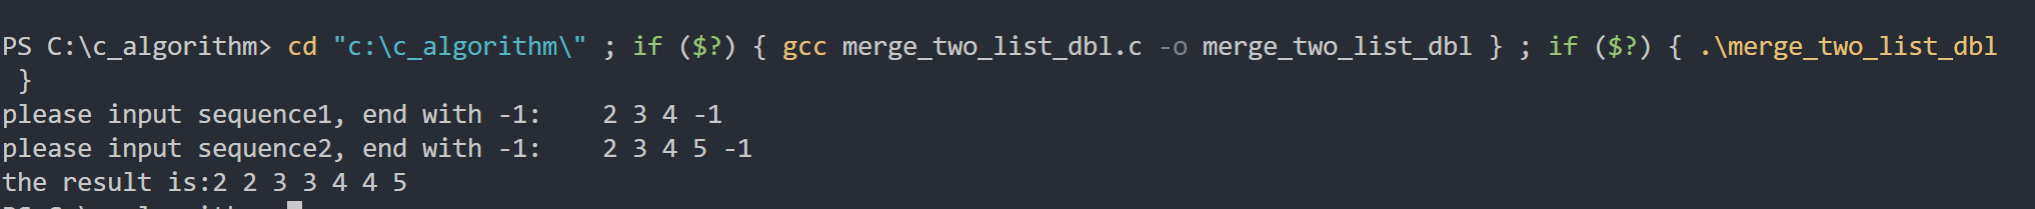
\includegraphics[scale=0.65]{dbl.png}
	\caption{运行结果1}
\end{figure}
\begin{figure}[!htbp]
	\centering
	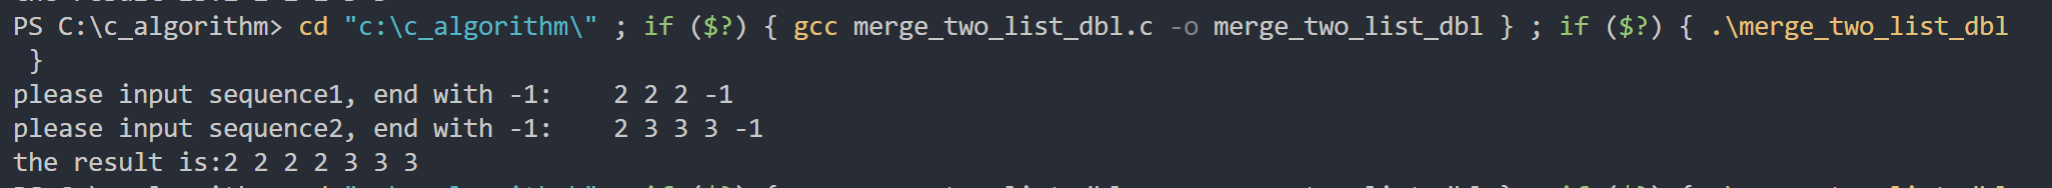
\includegraphics[scale=0.65]{test2.png}
	\caption{运行结果2}
\end{figure}
%	\begin{itemize}
%	\item 输入
%		\begin{itemize}
%			\item[ ]ACCBA
%			\item[ ]5
%			\item[ ]1 B
%			\item[ ]0 A
%			\item[ ]2 B
%			\item[ ]4 C
%			\item[ ]0 A
%		\end{itemize}
%	\item 输出
%		\begin{itemize}
%			\item[ ]ABCCBA
%			\item[ ]AABCCBA
%			\item[ ]AABBCCBA
%			\item[ ]-
%			\item[ ]A	
%		\end{itemize}
%	\end{itemize}
%	
%	\indent 更换多组数据测试均正确,其中$vector$版本以100分的成绩通过清华大学$Open\ Judge$测试。
	\subsection{算法时间复杂度}
    算法中的三个函数分别进行了一次while循环遍历整个链表,不存在嵌套循环情况,所以时间复杂度为$O(n)$
	\subsection{总结体会}
	\indent 第一次做这道题时我是用单链表做的,因为一开始没有看清题目的要求是双链表,成功的通过了测试,但不符合题目描述。之后我模仿着ppt使用双向循环链表,但是没有通过测试,debug结果为能够成功创建和输出双向链表,但是不能进行合并。于是在单链表上改成了双链表。这次因为电脑容量不足以安装$visual studio$在配置$vscode$的$debug$配置json环境花了很多时间。
\section{第二题}
\subsection{实验目的和内容}
	\indent 祖玛是一款曾经风靡全球的游戏,其玩法是:在一条轨道上初始排列着若干个彩色珠子,其中任意三个相邻的珠子不会完全同色。此后,你可以发射珠子到轨道上并加入原有序列中。一旦有三个或更多同色的珠子变成相邻,它们就会立即消失。这类消除现象可能会连锁式发生,其间你将暂时不能发射珠子。

\indent 开发商最近准备为玩家写一个游戏过程的回放工具。他们已经在游戏内完成了过程记录的功能,而回放功能的实现则委托你来完成。

\indent 游戏过程的记录中,首先是轨道上初始的珠子序列,然后是玩家接下来所做的一系列操作。你的任务是,在各次操作之后及时计算出新的珠子序列。
\subsection{输入和输出说明}
	\subsubsection{输入}
	\indent 第一行是一个由大写字母$’A’~’Z’$组成的字符串,表示轨道上初始的珠子序列,不同的字母表示不同的颜色。

\indent 第二行是一个数字$n$,表示整个回放过程共有$n$次操作。

\indent 接下来的$n$行依次对应于各次操作。每次操作由一个数字$k$和一个大写字母$\sum$描述,以空格分隔。其中,$\sum$为新珠子的颜色。若插入前共有$m$颗珠子,则$k\in[0, m]$表示新珠子嵌入之后(尚未发生消除之前)在轨道上的位序。
	\subsubsection{输出}
	\indent 输出共$n$行,依次给出各次操作(及可能随即发生的消除现象)之后轨道上的珠子序列。

\indent 如果轨道上已没有珠子,则以“$-$”表示。
	\subsubsection{样例}
	\begin{itemize}
	\item 输入
		\begin{itemize}
			\item[ ]ACCBA
			\item[ ]5
			\item[ ]1 B
			\item[ ]0 A
			\item[ ]2 B
			\item[ ]4 C
			\item[ ]0 A
		\end{itemize}
	\item 输出
		\begin{itemize}
			\item[ ]ABCCBA
			\item[ ]AABCCBA
			\item[ ]AABBCCBA
			\item[ ]-
			\item[ ]A	
		\end{itemize}
	\end{itemize}
\subsection{解题思路}
本题主要用了五个函数。\par
第一个建立双向链表函数,定义了头指针和尾指针并赋值$'-'$,并且用数组传参\par
第二个插入函数,就是找到某一个位置并进行插入\par
第三个是找到双向链表尾部,这个函数为删除,输出函数铺垫\par
第四个删除函数,需要注意的有两点:
\begin{itemize}
  \item 第一是需要找准删除的起点和终点
  \item 第二是需要讨论三种及以上的球的情况
\end{itemize}
第五个是输出函数,我们将双向链表赋值给数组并输出

\subsection{实验代码及注释}
\begin{lstlisting}
#include <stdio.h>
#include "string.h"
#include <stdlib.h>
#include <malloc.h>

#define Len 20000
#define Up (Len * 3 / 4)

typedef char ElemType;
typedef struct node //定义双向链表
{
    ElemType data; //数据域
    struct node *next;
    struct node *front; //指针域
} List, *pList;         //结点类型,结点指针

// pList pHead = (pList)malloc(sizeof(List));
// pList pTail = (pList)malloc(sizeof(List));
//常量表达式中不允许函数调用

char ans[Len + 5];
int forprt = 0;

pList creat(char *a, int n)
{
    /* n为参数个数,*a为传入参数*/
    int i;
    pList pHead = (pList)malloc(sizeof(List));
    pList pTail = (pList)malloc(sizeof(List)); //创建头指针和尾指针

    pList pt = pHead; // pt指向头指针

    pTail->front = pHead;
    pTail->next = NULL;
    pHead->next = pTail;
    pHead->front = NULL;             //创建空的双向链表
    pHead->data = pTail->data = '-'; //赋值为'-',表示轨道上已没有珠子

    for (i = 0; i < n; i++)
    {
        pList pNew = (pList)malloc(sizeof(List));
        pNew->data = a[i];  // 先通过gets得到数组储存字符串,然后通过数组来传值
        pNew->front = pt;
        pNew->next = pt->next;
        pt->next->front = pNew;
        pt->next = pNew;
        pt = pNew;  //移动pt指针
    }
    return pHead;
}

pList insert(int m, char ch, pList pHead)
{
    int i = -1; // i=-1.方便对位置零操作

    pList pt = pHead, pNew = (pList)malloc(sizeof(List));

    while (i++ < m)
        pt = pt->next; //找到带插入位置

    pNew->data = ch;
    pNew->next = pt;
    pNew->front = pt->front;
    pt->front->next = pNew;
    pt->front = pNew; //注意是插在找到位置的前面

    return pHead;
}

pList find_tail(pList pHead)
{
    pList pt = pHead->next;
    //while(!(pt->data == '-')) pt = pt ->next;
    while (pt->next != NULL)
        pt = pt->next;   //这两种方法都可以找到pTail
    return pt;
}

pList del(int m, pList pHead)
{
    pList pTail, point_tmp;
    pTail = find_tail(pHead);
    //获得ptail
    pList p1 = NULL, p2 = NULL, p3 = NULL, p4 = NULL, pt = pHead; //空指针最好赋值 NULL
    pList begin = pHead, end = pTail;
    int boo = 1; //gcc编译器不支持bool类型,所以用int表示逻辑
    int repeat, i = -1;

    // find position
    while (i++ < m - 2)
        pt = pt->next; // 找到插入位置前两个指针

    //init for 'begin' and 'end'
    begin = pt;
    end = pt;
    i = 0;
    while (i++ < 4 && end->next != pTail)
        end = end->next; //找到插入位置后两个指针

    while (boo && pt != pTail)
    {
        boo = 0; //判断有没有发生消除
        repeat = 1; //计数重复的个数
        while (pt != end) //pt在begin位置
        {
            pt = pt->next;

            if (pt->front->data == pt->data) //pt后移,如果data相同,就计数加一
                repeat++;
            else
                repeat = 1;

            if (repeat == 3)
            {
                boo = 1;
                if (pt->data == pt->next->data) //已经满足消除条件了,再看看能不能继续满足
                {
                    repeat++;
                    pt = pt->next;
                }

                if (repeat == 3)
                {
                    p3 = pt;
                    p2 = p3->front;
                    p1 = p2->front;
                    p1->front->next = p3->next;
                    p3->next->front = p1->front;
                    pt = pt->next; //消除这三个,将pt后移
                    free(p1);
                    free(p2);
                    free(p3);
                }
                else
                {
                    p4 = pt;
                    p3 = p4->front;
                    p2 = p3->front;
                    p1 = p2->front;
                    p1->front->next = p4->next;
                    p4->next->front = p1->front;
                    pt = pt->next; //消除这4个,将pt后移
                    free(p1);
                    free(p2);
                    free(p3);
                    free(p4);
                }

                break;
            }
        }

        if (boo && pt != pTail)
        {
            begin = pt;
            i = 0;
            while (i++ < 2 && begin->front != pHead)
                begin = begin->front;
            end = pt;
            i = 0;
            if (i++ < 1 && end->next != pTail)
                end = end->next;
            pt = begin; //将pt的begin和end指针归位
        }
    }
    return pHead;
}

pList show(int boo, pList pHead) //将双向链表的值存到数组便于输出
{

    pList pt = pHead->next;
    pList pTail = find_tail(pHead);

    if (pt == pTail)
        ans[forprt++] = '-'; //没有数
    else
    {
        while (pt->next != NULL)
        {
            ans[forprt++] = pt->data; //扩容并存data
            pt = pt->next;  //pt后移
        }
    }

    ans[forprt++] = '\n'; //输出需要有换行

    if (forprt >= Up || boo) //如果到尽头了
    {
        ans[forprt] = '\0'; //数组一定要以 \0 结尾
        printf("%s", ans); //输出
        forprt = 0;
    }
    return pHead; //其实不需要返回了
}

int main(void)
{
    char a[10005];
    int n, k;
    pList pHead = NULL;

    //printf("请输入初始队列\n");
    gets(a); // 初始的珠子序列
    //printf("请输入操作数");
    scanf("%d", &n); // 共有n次操作

    pHead = creat(a, strlen(a)); //创建对应初始的珠子序列的双向链表

    for (k = 0; k < n; k++)
    {
        int m;
        char ch;

        scanf("%d ", &m); //新的珠子位序

        ch = getchar(); // 插入珠子颜色

        // insert ch
        insert(m, ch, pHead);

        // delete all 3-same block, making it the right string
        del(m, pHead);

        // print the string
        show(k == n - 1 ? 1 : 0, pHead);
    }

    return 0;
}
\end{lstlisting}
\subsection{运行结果截图}
\begin{figure}[!htbp]
	\centering
	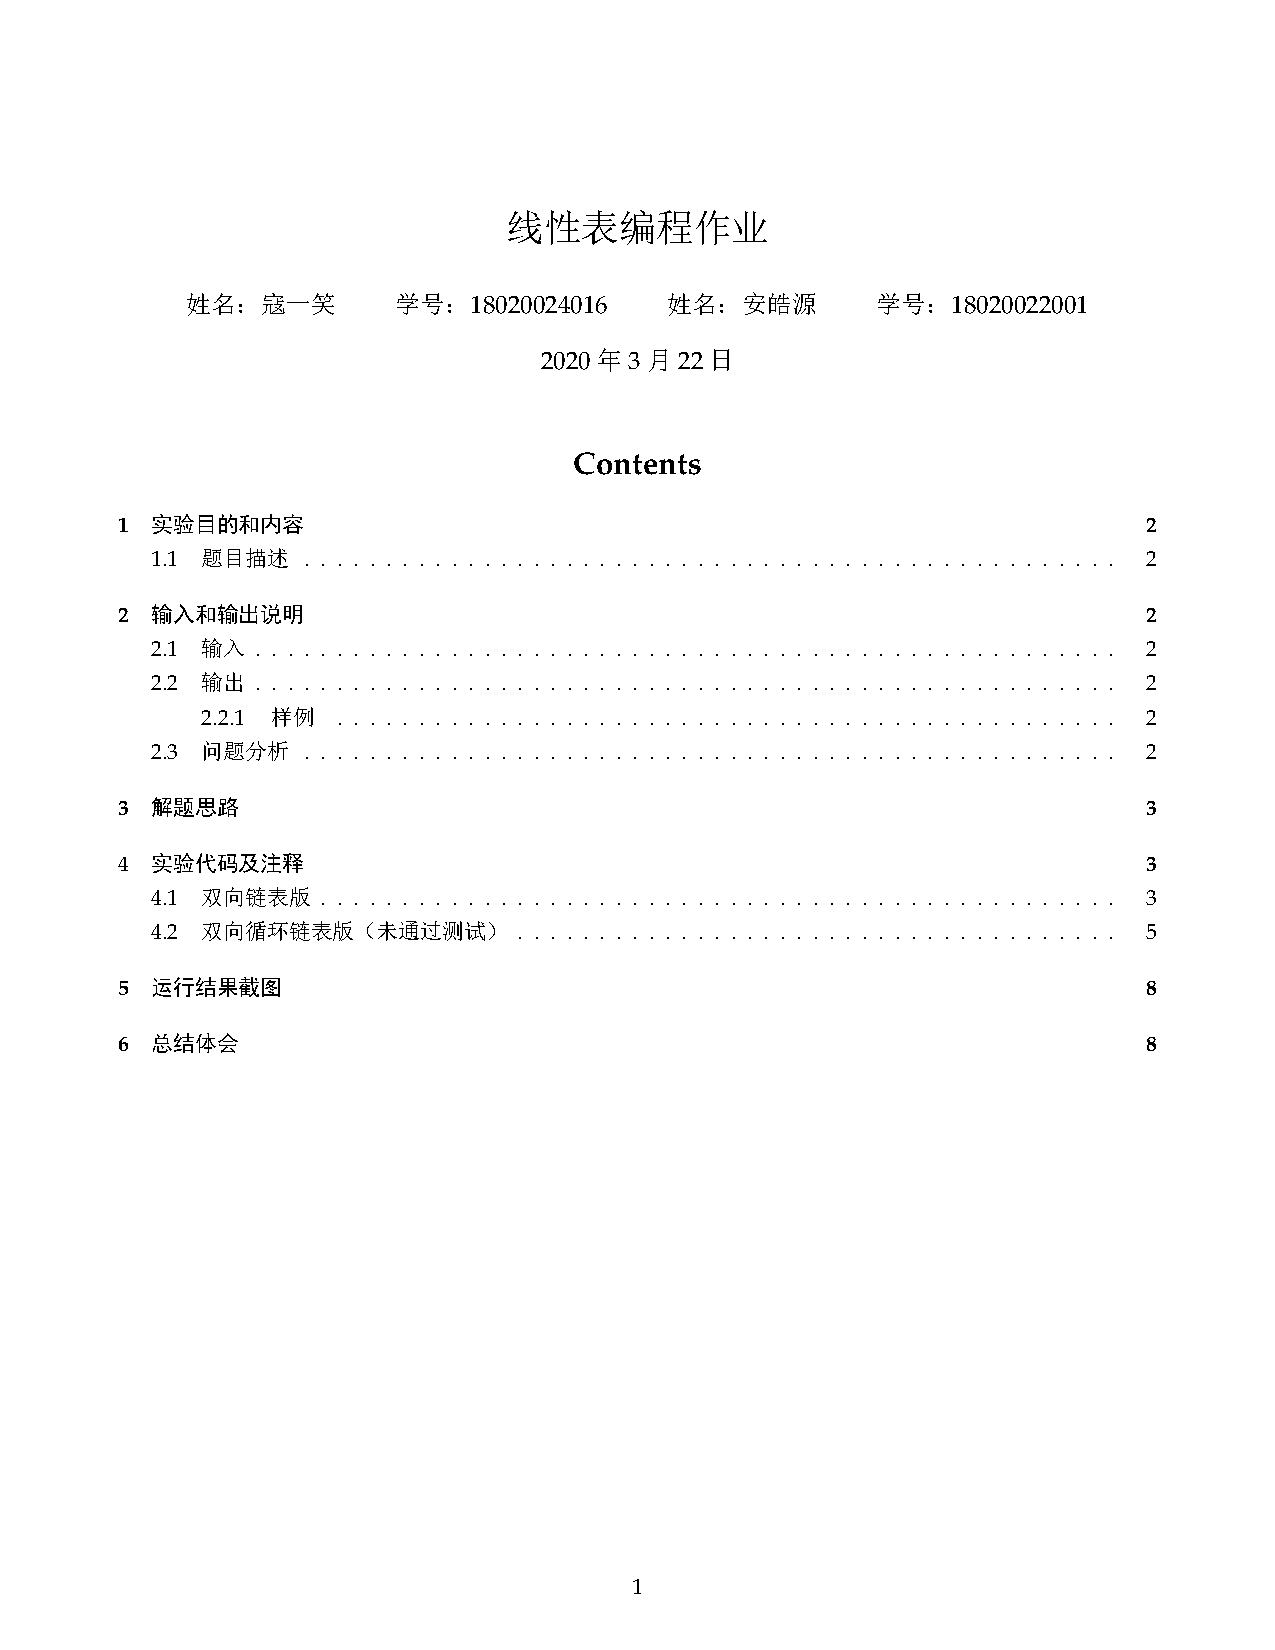
\includegraphics[scale=0.65]{zuma.png}
	\caption{运行结果}
\end{figure}
\subsection{总结体会}
主要复习了debug的基本操作,熟悉了双向链表的建立和删除操作。同时对于“实际问题”,需要分类讨论,考虑到多种情况。对于一些重复利用的操作可以写成函数方便调用
\appendix
\section{不用链表的zuma实现}
请看另一份报告
%\bibliography{ref.bib}
\end{document} 